\documentclass{article}
\usepackage[utf8]{inputenc}
\usepackage[margin=1.2in]{geometry}
\usepackage{hyperref}

\PassOptionsToPackage{usenames,dvipsnames,svgnames}{xcolor}  
\usepackage{tikz}
\usetikzlibrary{arrows,positioning,automata}

\usepackage{natbib}
\usepackage{graphicx}
\usepackage{amsmath}
\usepackage{listings}
\usepackage{xcolor}

\usepackage{tikz}
\usetikzlibrary{arrows.meta, positioning, shapes.geometric}

\definecolor{codegreen}{rgb}{0,0.6,0}
\definecolor{codegray}{rgb}{0.5,0.5,0.5}
\definecolor{codepurple}{rgb}{0.58,0,0.82}
\definecolor{backcolour}{rgb}{0.95,0.95,0.92}
\definecolor{deepblue}{rgb}{0,0,0.5}
\definecolor{deepred}{rgb}{0.6,0,0}
\definecolor{deepgreen}{rgb}{0,0.5,0}

\lstdefinestyle{mystyle}{
    backgroundcolor=\color{white},   
    commentstyle=\color{codegreen},
    keywordstyle=\color{deepblue},
    numberstyle=\tiny\color{codegray},
    stringstyle=\color{deepgreen},
    emph={Agent,__init__,act,self,union,exists, scope},
    emphstyle=\color{deepred},
    basicstyle=\ttfamily\footnotesize,
    breakatwhitespace=false,         
    breaklines=true,                 
    captionpos=b,                    
    keepspaces=true,                 
    numbers=left,                    
    numbersep=5pt,                  
    showspaces=false,                
    showstringspaces=false,
    showtabs=false,                  
    tabsize=3
}

\lstset{style=mystyle}

\title{\vspace{-2 cm} Universidade Federal de Ouro Preto \\ BCC 325 - Inteligência Artificial \\ Exame Especial \\ Prof. Rodrigo Silva}
\date{}


\begin{document}

\maketitle

\vspace{-1 cm}

\begin{itemize}

    \item O exame especial total é composto pelas questões marcadas com *.
    
    \item Na folha de prova indique qual exame especial você está fazendo. Parcial 1, 2 ou 3, ou total.
\end{itemize}

\section{Parcial 1}

\begin{enumerate}
    \item * Apresente o pseudocódigo do algoritmo de busca em largura e obtenha a expressão do seu custo de memória em termos da profundidade do grafo, $h$, e de seu \textit{branchinhg factor}, $b$ (número médio dos filhos de um nó). Atenção, o raciocínio utilizado para obter a expressão do custo deve ser demonstrado. 
    
    \item Apresente o pseudocódigo do algoritmo de busca em profundidade e obtenha a expressão do seu custo de memória em termos da profundidade do grafo, $h$, e de seu \textit{branchinhg factor}, $b$ (número médio dos filhos de um nó). Atenção, o raciocínio utilizado para obter a expressão do custo deve ser demonstrado.
    
    \item Apresente o pseudocódigo do algoritmo GAC (\textit{Generalized arc consistency}). Apresente também um exemplo de execução do pseudo-código apresentado. Atenção, o exemplo de execução deve corresponder ao pseudocódigo apresentado.  

\end{enumerate}

\section{Parcial 2}


\begin{enumerate}
    \item * Obtenha a expressão matricial para os coeficientes (pesos) de um modelo de regressão linear treinado com a técnica dos mínimos quadrados. Todos os passos da derivação da expressão devem ser apresentados e todas as variáveis utilizadas devem ser definidas.
    
    \item Apresente o pseudo-código do algoritmo utilizado para treinar um modelos de regressão logística. Explique cada linha. 

\end{enumerate}

\section{Parcial 3}

\begin{enumerate}

    \item  Considere a rede neural abaixo:
    
    \begin{figure}[!ht]
        \centering
        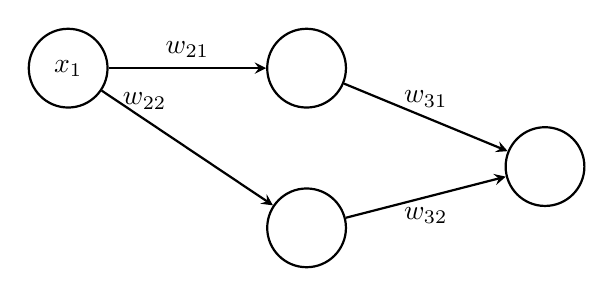
\begin{tikzpicture}[%
            neuron/.style={circle, draw, thick, minimum size=1cm},
            arrow/.style={->,>=stealth,thick}
        ]
        
        % Input neurons
        \node[neuron] (input1) at (0,0) {$x_1$};
        %\node[neuron] (input2) [below=of input1] {$x_2$};
        
        % Hidden layer neurons
        \node[neuron] (hidden1) [right=2cm of input1] {};
        \node[neuron] (hidden2) [below=of hidden1] {};
        
        % Output neuron
        \node[neuron] (output) [right=2cm of hidden1, yshift=-1.25cm] {};
        
        % Connect input layer to hidden layer
        \draw[arrow] (input1) -- (hidden1) node[midway, above] {$w_{21}$};
        \draw[arrow] (input1) -- (hidden2) node[near start, above] {$w_{22}$};
        %\draw[arrow] (input2) -- (hidden1) node[near start, below] {$w_{12}$};
        %\draw[arrow] (input2) -- (hidden2) node[midway, below] {$w_{22}$};
        
        % Connect hidden layer to output layer
        \draw[arrow] (hidden1) -- (output) node[midway, above] {$w_{31}$};
        \draw[arrow] (hidden2) -- (output) node[midway, below] {$w_{32}$};
        
        \end{tikzpicture}
    \end{figure}

    Esta rede não possui termos de viés (bias) e tem como funções de ativação a função ReLU (Rectified Linear Unit) que pode ser definida como:

    \begin{equation}
        \text{ReLU}(x) = \max(0, x)
    \end{equation}

    A derivada da ReLU é definida como:

    \begin{equation}
            \frac{d}{dx}(\text{ReLU}(x)) =
            \begin{cases}
            1 & \text{if } x > 0 \\
            0 & \text{if } x \leq 0
            \end{cases}            
    \end{equation}

    Obtenha o gradiente do erro quadrado em relação aos pesos da rede. Todos os passos da derivação da gradiente devem ser apresentados.

    \item * Apresente o pseudocódigo dos algoritmos de prova bottom-up e top-down.


\end{enumerate}


\end{document}

